\begin{enumerate}
	\item L'administrateur se connecte au site avec ses identifiant. 
	\item Un nouveau bouton de navigation apparait dans la bar de navigation. 
	\item L'administrateur clique sur le bouton \textit{Admin}
	\item Il sélectionne \textit{Abonnement} dans le menu déroulant. 
	\item L'administrateur atterris sur la page de gestion des type des utilisateurs. 
	\item Il clique sur le bouton supprimer
	\item Une fenêtre de confirmation apparait. 
	\item Il clique sur \textit{OUI!} 
\end{enumerate}

\newpage
\begin{figure}[h]
	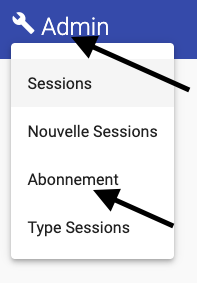
\includegraphics[width=0.4\textwidth,center]{Figures/us15-1}
	\caption{Menu de l'administrateur}
\end{figure}

\vspace{\baselineskip}
\begin{figure}[h]
	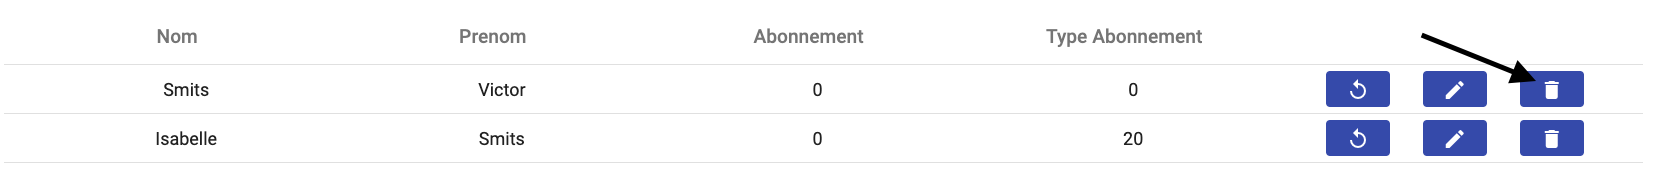
\includegraphics[width=\textwidth,center]{Figures/us15-2}
	\caption{Bouton de suppression de l'utilisateur}
\end{figure}

\vspace{\baselineskip}
\begin{figure}[h]
	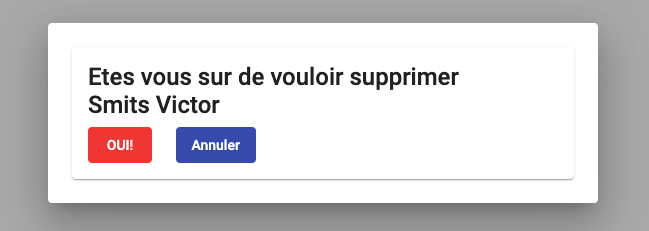
\includegraphics[width=0.5\textwidth,center]{Figures/us15-3}
	\caption{Fenêtre de confirmation de suppression}
\end{figure}

\subsubsection{Script concerné}
	\begin{itemize}
		\item \href{https://github.com/victorsmits/Aquabike/blob/master/backend/src/Controller/API/AbonnementControllerApi.php}{AbonnementControllerApi.php}
		\item \href{https://github.com/victorsmits/Aquabike/blob/master/backend/src/Entity/Person.php}{Person.php}
		\item \href{https://github.com/victorsmits/Aquabike/blob/master/frontend/src/app/type-session/del-abo.component.ts}{del-abo.component.ts}
		\item \href{https://github.com/victorsmits/Aquabike/blob/master/frontend/src/app/type-session/del-abo.component.html}{del-abo.component.html}
	\end{itemize}
